\documentclass[tikz,border=4pt]{standalone}
\usepackage[T1]{fontenc}
\usepackage[utf8]{inputenc}
\usepackage{tikz}
\usetikzlibrary{arrows.meta,positioning,calc,fit}

% ------------------------------------------------------------
% Palette consistent with approved TFM figures
% ------------------------------------------------------------
\definecolor{archdark}{HTML}{263142}
\definecolor{archslate}{HTML}{64748B}
\definecolor{archlight}{HTML}{F8FAFC}
\definecolor{archmuted}{HTML}{EEF2F7}
\definecolor{subsysTUFill}{HTML}{DCEAF7}
\definecolor{subsysFUFill}{HTML}{DDEED8}
\definecolor{subsysATMFill}{HTML}{F7E6B8}
\definecolor{subsysACTFill}{HTML}{F3D8DE}
\definecolor{subsysELECFill}{HTML}{E4DDF2}
\definecolor{subsysCTRLFill}{HTML}{D6ECEF}
\definecolor{subsysEXPFill}{HTML}{E5E7EB}
\definecolor{flexColor}{HTML}{C2185B}
\definecolor{extColor}{HTML}{007C91}

\tikzset{
  >={Latex[length=2.4mm,width=1.5mm]},
  base/.style={draw=archdark, rounded corners=3pt, line width=0.82pt,
               font=\small\sffamily, text=archdark, align=center,
               inner xsep=4pt, inner ysep=3pt},
  callout/.style={base, fill=white, minimum width=3.05cm, minimum height=0.88cm},
  routeLabel/.style={font=\scriptsize\bfseries\sffamily, fill=white,
                    inner xsep=2.4pt, inner ysep=1.0pt},
  smallLabel/.style={font=\scriptsize\sffamily, text=archdark, align=center},
  guide/.style={draw=archslate!65, dashed, line width=0.7pt},
  flexroute/.style={->, draw=flexColor, line width=2.1pt},
  extroute/.style={->, draw=extColor, line width=2.1pt},
  leader/.style={->, draw=archdark, line width=0.8pt}
}

\begin{document}
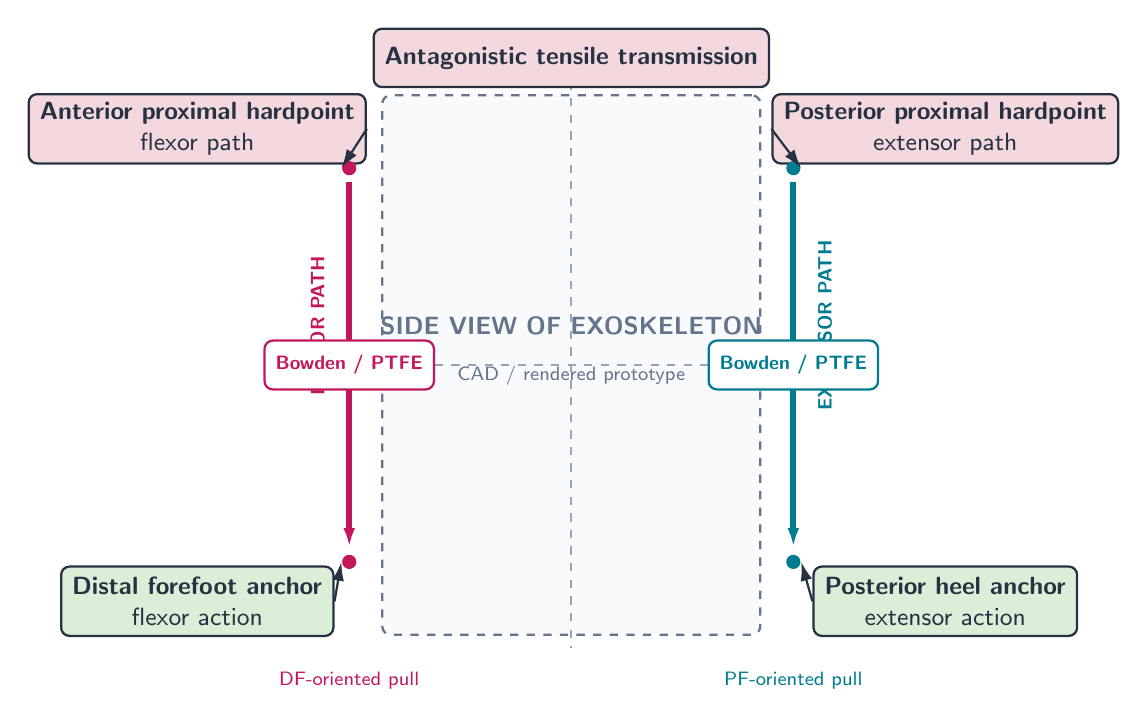
\begin{tikzpicture}[font=\sffamily]

% ------------------------------------------------------------
% CENTRAL PLACEHOLDER: replace this group with lateral CAD/render
% in Inkscape while preserving its bounding box/alignment.
% ------------------------------------------------------------
\node[base, fill=archlight, dashed, draw=archslate,
      minimum width=4.8cm, minimum height=6.85cm] (exo) at (7.0,4.55) {};
\node[font=\bfseries\small\sffamily, text=archslate] at (7.0,5.05)
{SIDE VIEW OF EXOSKELETON};
\node[smallLabel, text=archslate] at (7.0,4.42)
{CAD / rendered prototype};

% subtle alignment guides
\draw[guide] (7.0,8.15) -- (7.0,0.95);
\draw[guide] (4.0,4.55) -- (10.0,4.55);

% ------------------------------------------------------------
% PROXIMAL CONNECTIONS
% ------------------------------------------------------------
\node[callout, fill=subsysACTFill] (proxF) at (2.25,7.55)
{\textbf{Anterior proximal hardpoint}\\flexor path};
\node[callout, fill=subsysACTFill] (proxE) at (11.75,7.55)
{\textbf{Posterior proximal hardpoint}\\extensor path};

% anchor dots near central CAD boundary
\fill[flexColor] (4.18,7.05) circle (0.09cm);
\fill[extColor]  (9.82,7.05) circle (0.09cm);
\draw[leader] (proxF.east) -- (4.08,7.05);
\draw[leader] (proxE.west) -- (9.92,7.05);

% ------------------------------------------------------------
% DISTAL CONNECTIONS
% ------------------------------------------------------------
\node[callout, fill=subsysFUFill] (distF) at (2.25,1.55)
{\textbf{Distal forefoot anchor}\\flexor action};
\node[callout, fill=subsysFUFill] (distE) at (11.75,1.55)
{\textbf{Posterior heel anchor}\\extensor action};

\fill[flexColor] (4.18,2.05) circle (0.09cm);
\fill[extColor]  (9.82,2.05) circle (0.09cm);
\draw[leader] (distF.east) -- (4.08,2.05);
\draw[leader] (distE.west) -- (9.92,2.05);

% ------------------------------------------------------------
% ANTAGONISTIC ROUTES
% FLEX = anterior / forefoot side, EXT = posterior / heel side
% ------------------------------------------------------------
\draw[flexroute] (4.18,6.88) -- (4.18,2.24);
\draw[extroute]  (9.82,6.88) -- (9.82,2.24);

\node[routeLabel, text=flexColor, rotate=90] at (3.78,5.05) {FLEXOR PATH};
\node[routeLabel, text=extColor, rotate=90] at (10.22,5.05) {EXTENSOR PATH};

\node[base, fill=white, draw=flexColor, text=flexColor,
      minimum width=2.0cm, minimum height=0.62cm,
      font=\scriptsize\bfseries\sffamily] at (4.18,4.55)
{Bowden / PTFE};
\node[base, fill=white, draw=extColor, text=extColor,
      minimum width=2.0cm, minimum height=0.62cm,
      font=\scriptsize\bfseries\sffamily] at (9.82,4.55)
{Bowden / PTFE};

% ------------------------------------------------------------
% Direction / action semantics
% ------------------------------------------------------------
\node[base, fill=subsysACTFill, minimum width=3.4cm, minimum height=0.74cm] at (7.0,8.45)
{\textbf{Antagonistic tensile transmission}};

\node[smallLabel, text=flexColor, anchor=north] at (4.18,0.78)
{DF-oriented pull};
\node[smallLabel, text=extColor, anchor=north] at (9.82,0.78)
{PF-oriented pull};

\end{tikzpicture}
\end{document}
